%!TEX TS-program = xelatex 
%!TEX TS-options = -output-driver="xdvipdfmx -q -E"
%!TEX encoding = UTF-8 Unicode
%
%  summary_4
%
%  Created by Mark Eli Kalderon on 2009-02-24.
%

\documentclass[11pt]{article} 

% Definitions
\newcommand\myauthor{Mark Eli Kalderon} 
\newcommand\mytitle{Oxford Philosophy of Perception:}
\newcommand\mysubtitle{Prichard and the Theory of Appearance}

% Packages
\usepackage{url}
\usepackage{txfonts}
\usepackage{color}
\definecolor{myblue}{rgb}{0.8,0.8,1}

% Define discussion environment
\makeatletter\newenvironment{discussion}{%
   \noindent\begin{lrbox}{\@tempboxa}\begin{minipage}{\columnwidth}\setlength{\parindent}{1em}}{\end{minipage}\end{lrbox}%
   \colorbox{myblue}{\usebox{\@tempboxa}}
}\makeatother

% XeTeX
\usepackage[cm-default]{fontspec}
\usepackage{xltxtra,xunicode}
\defaultfontfeatures{Scale=MatchLowercase,Mapping=tex-text}
\setmainfont{Hoefler Text}
\setsansfont{Gill Sans}
\setmonofont{Inconsolata}

% Title Information
\title{\mytitle\\
\mysubtitle}
\author{\myauthor} 
\date{} % Leave blank for no date, comment out for most recent date

% PDF Stuff
\usepackage[plainpages=false, pdfpagelabels, bookmarksnumbered, backref, pdftitle={\mytitle}, pagebackref, pdfauthor={\myauthor}, xetex, colorlinks=true, linkcolor=gray, urlcolor=gray]{hyperref}

%%% BEGIN DOCUMENT
\begin{document}

% Title Page
\maketitle

% Layout Settings
\setlength{\parindent}{1em}

% Main Content

\begin{figure}[htbp]
    \centering
        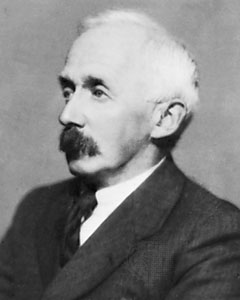
\includegraphics[scale=1]{../../graphics/prichard.jpg}
    \caption{H.A. Prichard}
    \label{fig:prichard}
\end{figure}

\section{The Theory of Appearing} % (fold)
\label{sec:the_theory_of_appearing}
For Prichard, canonical appearance-attributions take the following form:
    \begin{quote}
        \( o \) appears \( F \)
    \end{quote}
Prichard makes five central claims about appearances described by canonical appearance-attributions:
    \begin{enumerate}
        \item \( o \) is an external body located in space.
        \item Appearance is relational. An appearance is the presentation of \( o \)---it is \( o \) appearing \( F \) to a subject \( S \).
        \item The predicate \( F \) has spatial conditions of application---it is intelligibly applied only to spatial bodies.
        \item The external spatial body \( o \) is the object of the perception in virtue of which \( o \) appears.
        \item Our perception of \( o \) enables us to apprehend \( o \) and so come to know about it.
    \end{enumerate}
% section the_theory_of_appearing (end)

\end{document}
